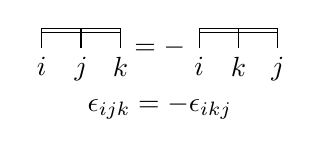
\begin{tikzpicture}
    \draw
    (0,1)--(1,1)
    (0,.95)--(1,.95)
    (0,1)--(0,.75) node[anchor=north]{$i$}
    (.5,1)--(.5,.75) node[anchor=north]{$j$}
    (1,1)--(1,.75) node[anchor=north]{$k$}
    ;
    \node[anchor=center]at(1.5,.75){$=-$};
    \draw
    (2,1)--(3,1)
    (2,.95)--(3,.95)
    (2,1)--(2,.75) node[anchor=north]{$i$}
    (2.5,1)--(2.5,.75) node[anchor=north]{$k$}
    (3,1)--(3,.75) node[anchor=north]{$j$}
    ;
    \node[anchor=center]at(1.5,0){$\epsilon_{ijk}=-\epsilon_{ikj}$};
\end{tikzpicture}
